\documentclass[11pt]{article}
\usepackage[spanish]{babel}
\usepackage[T1]{fontenc}
\usepackage{amsmath,amsfonts,amssymb,amsthm}
\usepackage{amsfonts}
\usepackage{graphicx}
\usepackage{geometry}
\usepackage{newpxtext,euler}
\usepackage{float}
\usepackage{xcolor}
\usepackage{geometry}
 \geometry{
 a4paper,
 total={170mm,245mm},
 left=20mm,
 top=30mm,
 }
\pagestyle{empty}

\title{Taller III}

\author{Bourbaki}
\date{\today}


\begin{document}

\maketitle


\begin{enumerate}
    \item Demuestre que \( A \subset \mathbb{C} \) es compacto si y solo si es acotado y cerrado.

    \begin{proof}
    Supongamos que $A$ es compacto, si $A$ no es acotado entonces para todo $n\in \mathbb{N}$, existe $z_n\in A$ tal que $|z_n|>n$, por tanto $\{z_n\}$ no tiene punto de acumulación ya que... suponga que $z_0$ es un punto de acumulación, sea $m>2|z_0|$, es claro que $|z_0|>0$ ya que en caso contrario $z_0=0$, así pues $|z_n-z_0|=|z_n|>n$ y por lo tanto $z_0$ no sería punto de acumulación. En este caso $|z_m-z_0|\geq |z_m|-|z_0|>2|z_0|-|z_0|=|z_0|$, contradice que ese coso es punto límite. Entonces es acotado.\\

    Sea $z_0\in \overline{A}$, dado $n$, existe $z_n\in A$ tal que $|z_n-z_0|<\dfrac{1}{n}$, así $\{z_n\}$ converge a $z_0$. Como $A$ es compacto existe una subsucesión convergente en A, es claro que este límite debe ser $z_0$, así $z_0\in A$, con lo cual $A$ es cerrado.\\

    El recíproco tengo pereza



    \end{proof}

    \item Sea \( K \subset \mathbb{C} \) compacto. Sean \( K_1 \supseteq K_2 \supseteq K_3 \supseteq \cdots \) una sucesión de subconjuntos de \( K \) no vacíos, tales que \( K_n \supseteq K_{n+1} \). Demostrar que la intersección de todos los \( K_n, n = 1, 2, 3, \ldots \) es no vacía.\\

    Pues lo que pasa es que eso siempre es  fácil allí porque usted llega y coge el conjunto $\left(0,\dfrac{1}{n}\right)$ $n\in \mathbb{N}$, note que ese conjunto está contenido en $[0,1]$ que es compacto, y pues si usted considera la intersección de esos coyos, eso le da vacío siono?

    \item Encontrar la imagen de las regiones:
    \[1 < | \operatorname{Im}(z) | \leq 2\]

    \begin{figure}[H]
    \centering
    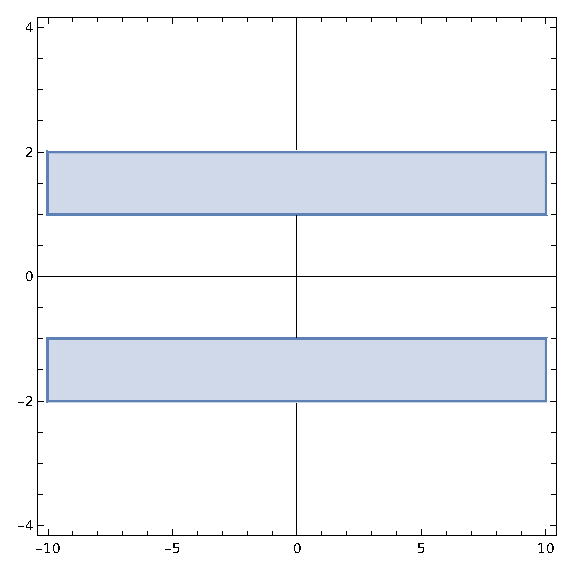
\includegraphics[scale=0.8]{P3-1.eps}
    \end{figure}

    \[|z| < 1\]

    \begin{figure}[H]
    \centering
    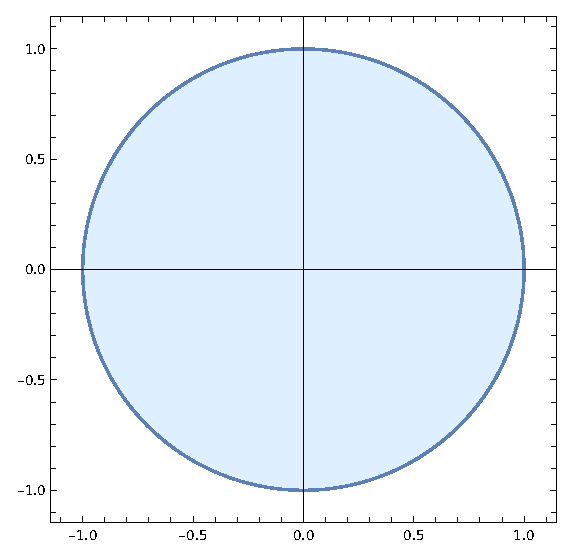
\includegraphics[scale=0.8]{P3-2.eps}
    \end{figure}

    bajo las aplicaciones:
    \begin{enumerate}
        \item \( f(z) = z^2 \)\\

        Sea $z=x+yi$, entonces $z^2=x^2-y^2+2xyi$, sean $u(x,y)=x^2-y^2$ y $v(x,y)=2xy$ las funciones parte real e imaginaria, esto es

        $$x=\frac{v}{2y}$$ 

        reemplazando en la ecuación de arriba se obtiene que 

        $$u=\frac{v^2}{4y^2}-y^2$$

        si uno reemplaza en $-2$ y $-1$ obtiene las ecuaciones de dos parábolas, pero pues usted tiene que girar la cabeza  para verlo bien

        $$u=\frac{v^2}{16}-4\quad u=\frac{v^2}{4}-1$$

       \begin{figure}[H]
        \centering
        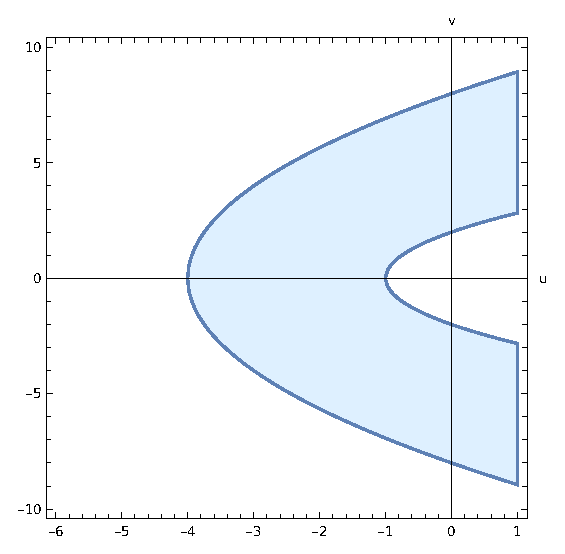
\includegraphics[scale=0.86]{S1.eps}
        \end{figure}     

        Para el caso $|z|<1$ nos deja la misma bola porque dado $z=re^{i\theta}$ entonces $z^2=r^2e^{i2\theta}$ por lo que nos queda la misma circunferencia, dado que si $0\leq r<1$ entonces $0\leq r^2<1$
        \item \( f(z) = \dfrac{2z + i}{z + 1} \)\\

        \textcolor{red}{Esto lo irá a hacer su madre y con su madre me refiero al Santiago xd.}

    \end{enumerate}

    \item  Sea \( f(z) = \dfrac{z - i}{z + i} \), hallar la imagen por \( f \) de:
    \begin{enumerate}
        \item El semiplano superior.
        \item La semirecta \( it; t \geq 0 \).
        \item La recta \( it; t \in \mathbb{R} \).
        \item \( |z - 1| = 1 \).
        \item \( |z| = 2; \operatorname{Im}(z) \geq 0 \).
    \end{enumerate}

    \item Sea \( A = \{ z \in \mathbb{C} : -\infty < \operatorname{Im}(z) \leq \alpha \} \). Si \( f(z) = e^z \), hallar \( f(A) \).

    \item Sea \( A = \{ z \in \mathbb{C} : |\operatorname{Re}(z)| < \frac{\pi}{2}, \operatorname{Im}(z) > 0 \} \). Si \( f(z) = \sin(z) \), hallar \( f(A) \).

    \item Determine completamente la proyección estereográfica (que lleva la esfera de Riemann en el plano complejo). Es decir, hallar explícitamente \( T \) y \( T^{-1} \).

    \item Demostrar que la proyección estereográfica preserva círculos. La imagen directa o inversa de una circunferencia es una circunferencia.
\end{enumerate}

\end{document}